\documentclass[11pt]{article}
\usepackage{graphicx}
\usepackage{geometry}
\geometry{margin=1in}

\title{BNNs Project Report}
\date{}

\begin{document}
\maketitle

\section{Overview}
This project compares Bayesian neural network methods:
\begin{itemize}
\item Laplace approximation (post-hoc)
\item Bayesian-Torch (SVI with Flipout)
\item MAP baseline
\end{itemize}

The project has 7 notebooks covering 2 datasets.

\section{Datasets}

\subsection{Sinusoidal Regression}
\begin{itemize}
\item 1D function: sin(x) + noise
\item 150 train points, 500 test points
\item Known noise sigma = 0.3
\item Used in 4 notebooks
\end{itemize}

\subsection{Two Moons Classification}
\begin{itemize}
\item 10k samples, noise = 0.3
\item 60/20/20 train/val/test split
\item StandardScaler normalization
\item Used in 2 notebooks
\end{itemize}

\subsection{PovertyMap (WILDS)}
\begin{itemize}
\item Satellite imagery, 8-channel
\item ResNet-18 adapted architecture
\item 5 country folds (A to E)
\item ID vs OOD evaluation
\item Used in 1 notebook
\end{itemize}

\section{Libraries}

\subsection{Laplace-Torch}
\begin{itemize}
\item from laplace import Laplace
\item Approximates posterior as Gaussian around MAP
\item Uses Hessian of loss at MAP weights
\item GLM predictive for closed-form variance
\item Supports diag, kron, full Hessian
\item Hyperparameters tuned via marglik or grid search
\end{itemize}

\subsection{Bayesian-Torch}
\begin{itemize}
\item from bayesian\_torch.models.dnn\_to\_bnn import dnn\_to\_bnn, get\_kl\_loss
\item Learns posterior via SVI during training
\item Flipout estimator for low-variance gradients
\item MOPED initialization from MAP weights
\item ELBO loss: MSE + KL/batch\_size
\item MC sampling for predictive distribution
\end{itemize}

\section{Notebooks}

\subsection{bnn\_laplace\_visualization.ipynb}
\begin{itemize}
\item Laplace on sinusoid regression
\item MAP training, Hessian fit, marglik optimization
\item Predictions with uncertainty bands
\item Parametric study with noise levels 0.1, 0.3, 0.5
\item Saves model state and predictions
\end{itemize}

\subsection{two\_moons\_laplace.ipynb}
\begin{itemize}
\item Laplace on Two Moons classification
\item Three Hessian types: diag, full, kron
\item Grid search and marglik tuning
\item 16 figures saved to figures/
\item Metrics exported to CSV
\end{itemize}

\subsection{bnn\_bayesian\_torch.ipynb}
\begin{itemize}
\item Bayesian-Torch on sinusoid
\item MOPED init from MAP weights
\item Flipout layers, ELBO fine-tuning
\item 100 MC samples for uncertainty
\item Epistemic = 0.97, Aleatoric = 0.30
\end{itemize}

\subsection{bnn\_bayesian\_torch1.ipynb}
\begin{itemize}
\item Same as above (duplicate/backup)
\item Same pipeline and results
\end{itemize}

\subsection{bnn\_comparison\_povertymap.ipynb}
\begin{itemize}
\item Laplace vs Bayesian-Torch on PovertyMap
\item ResNet-18, 5-fold cross-validation
\item ID and OOD generalization
\item Metrics: MSE, NLL, Calibration Error
\item Laplace: 12x faster training, lower NLL
\end{itemize}

\subsection{bnn\_comparison\_sinusoid.ipynb}
\begin{itemize}
\item Three-way: MAP, Laplace, Bayesian-Torch
\item Metrics: RMSE, NLL, Calibration Error
\item Bayesian-Torch best RMSE (1.09)
\item Laplace highest epistemic (1.71)
\item Results exported to CSV
\end{itemize}

\subsection{two\_moons\_bayesian.ipynb}
\begin{itemize}
\item Bayesian-Torch on Two Moons
\item Flipout vs BBB/Reparameterization
\item Metrics: Accuracy, NLL, Brier, ECE, ROC-AUC
\item Uncertainty decomposition: epistemic vs aleatoric
\item 5 figures saved
\end{itemize}

\section{Metrics}

\begin{itemize}
\item RMSE: sqrt(mean((y - y\_pred)\textasciicircum2))
\item NLL: negative log likelihood of predictions
\item Calibration Error: confidence vs accuracy alignment
\item ECE: Expected Calibration Error
\item Brier Score: MSE of predicted probabilities
\item Epistemic Uncertainty: model uncertainty
\item Aleatoric Uncertainty: data noise
\item Training Time: wall-clock for fitting
\item Inference Time: wall-clock for predictions
\end{itemize}

\section{Figures}

\begin{figure}[h]
\centering
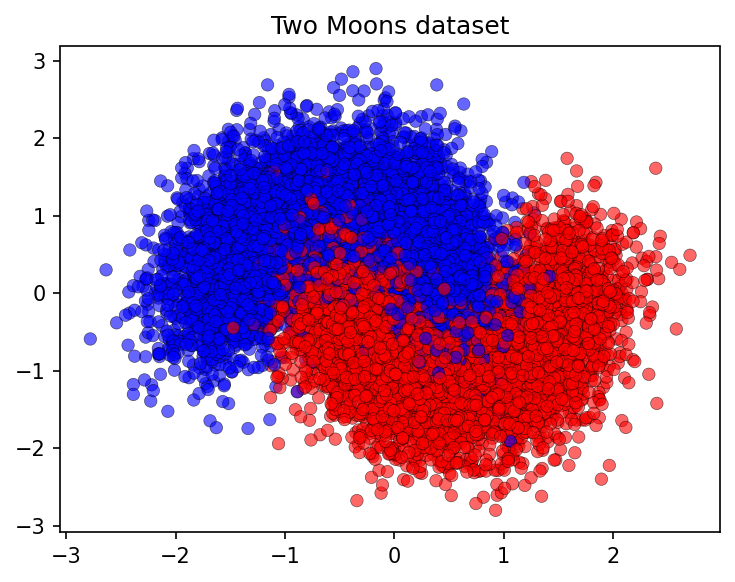
\includegraphics[width=0.45\textwidth]{./laplace_torch/figures/01_raw_dataset.png}
\caption{Two Moons raw dataset}
\end{figure}

\begin{figure}[h]
\centering
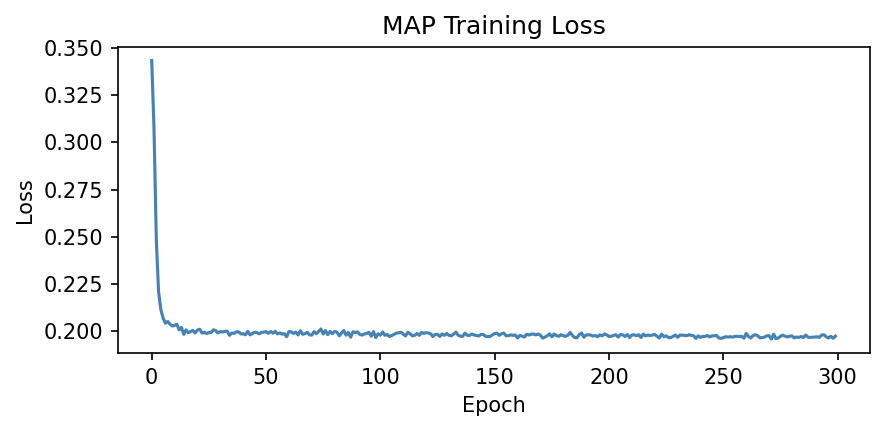
\includegraphics[width=0.45\textwidth]{./laplace_torch/figures/02_map_training_loss.png}
\caption{MAP training loss}
\end{figure}

\begin{figure}[h]
\centering
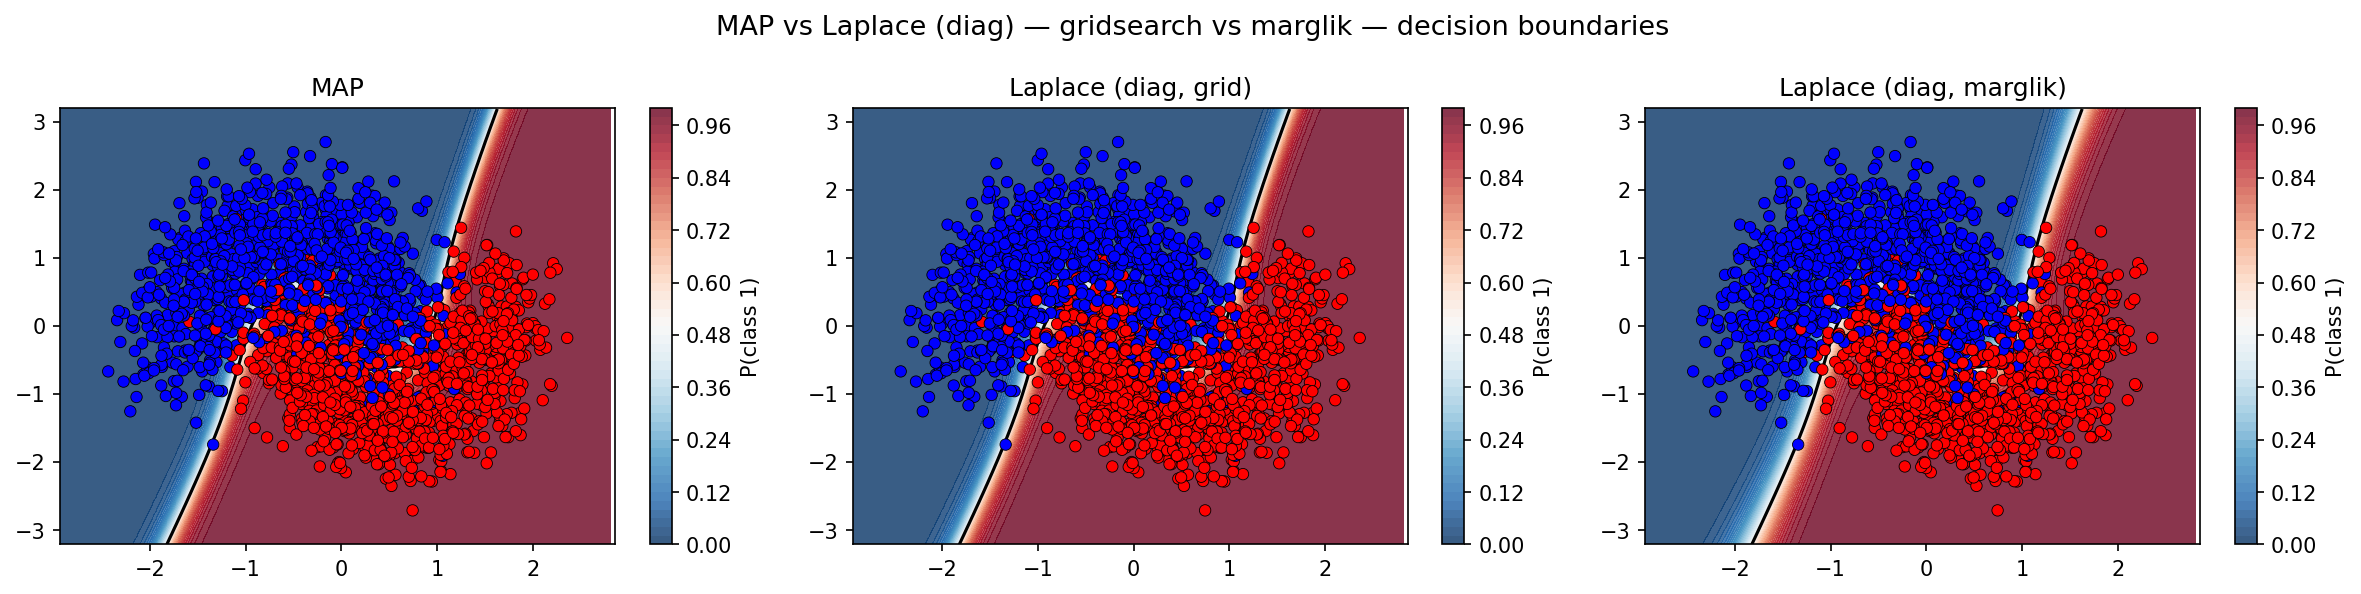
\includegraphics[width=0.45\textwidth]{./laplace_torch/figures/07_three_way_boundary.png}
\caption{Three-way boundary comparison}
\end{figure}

\begin{figure}[h]
\centering
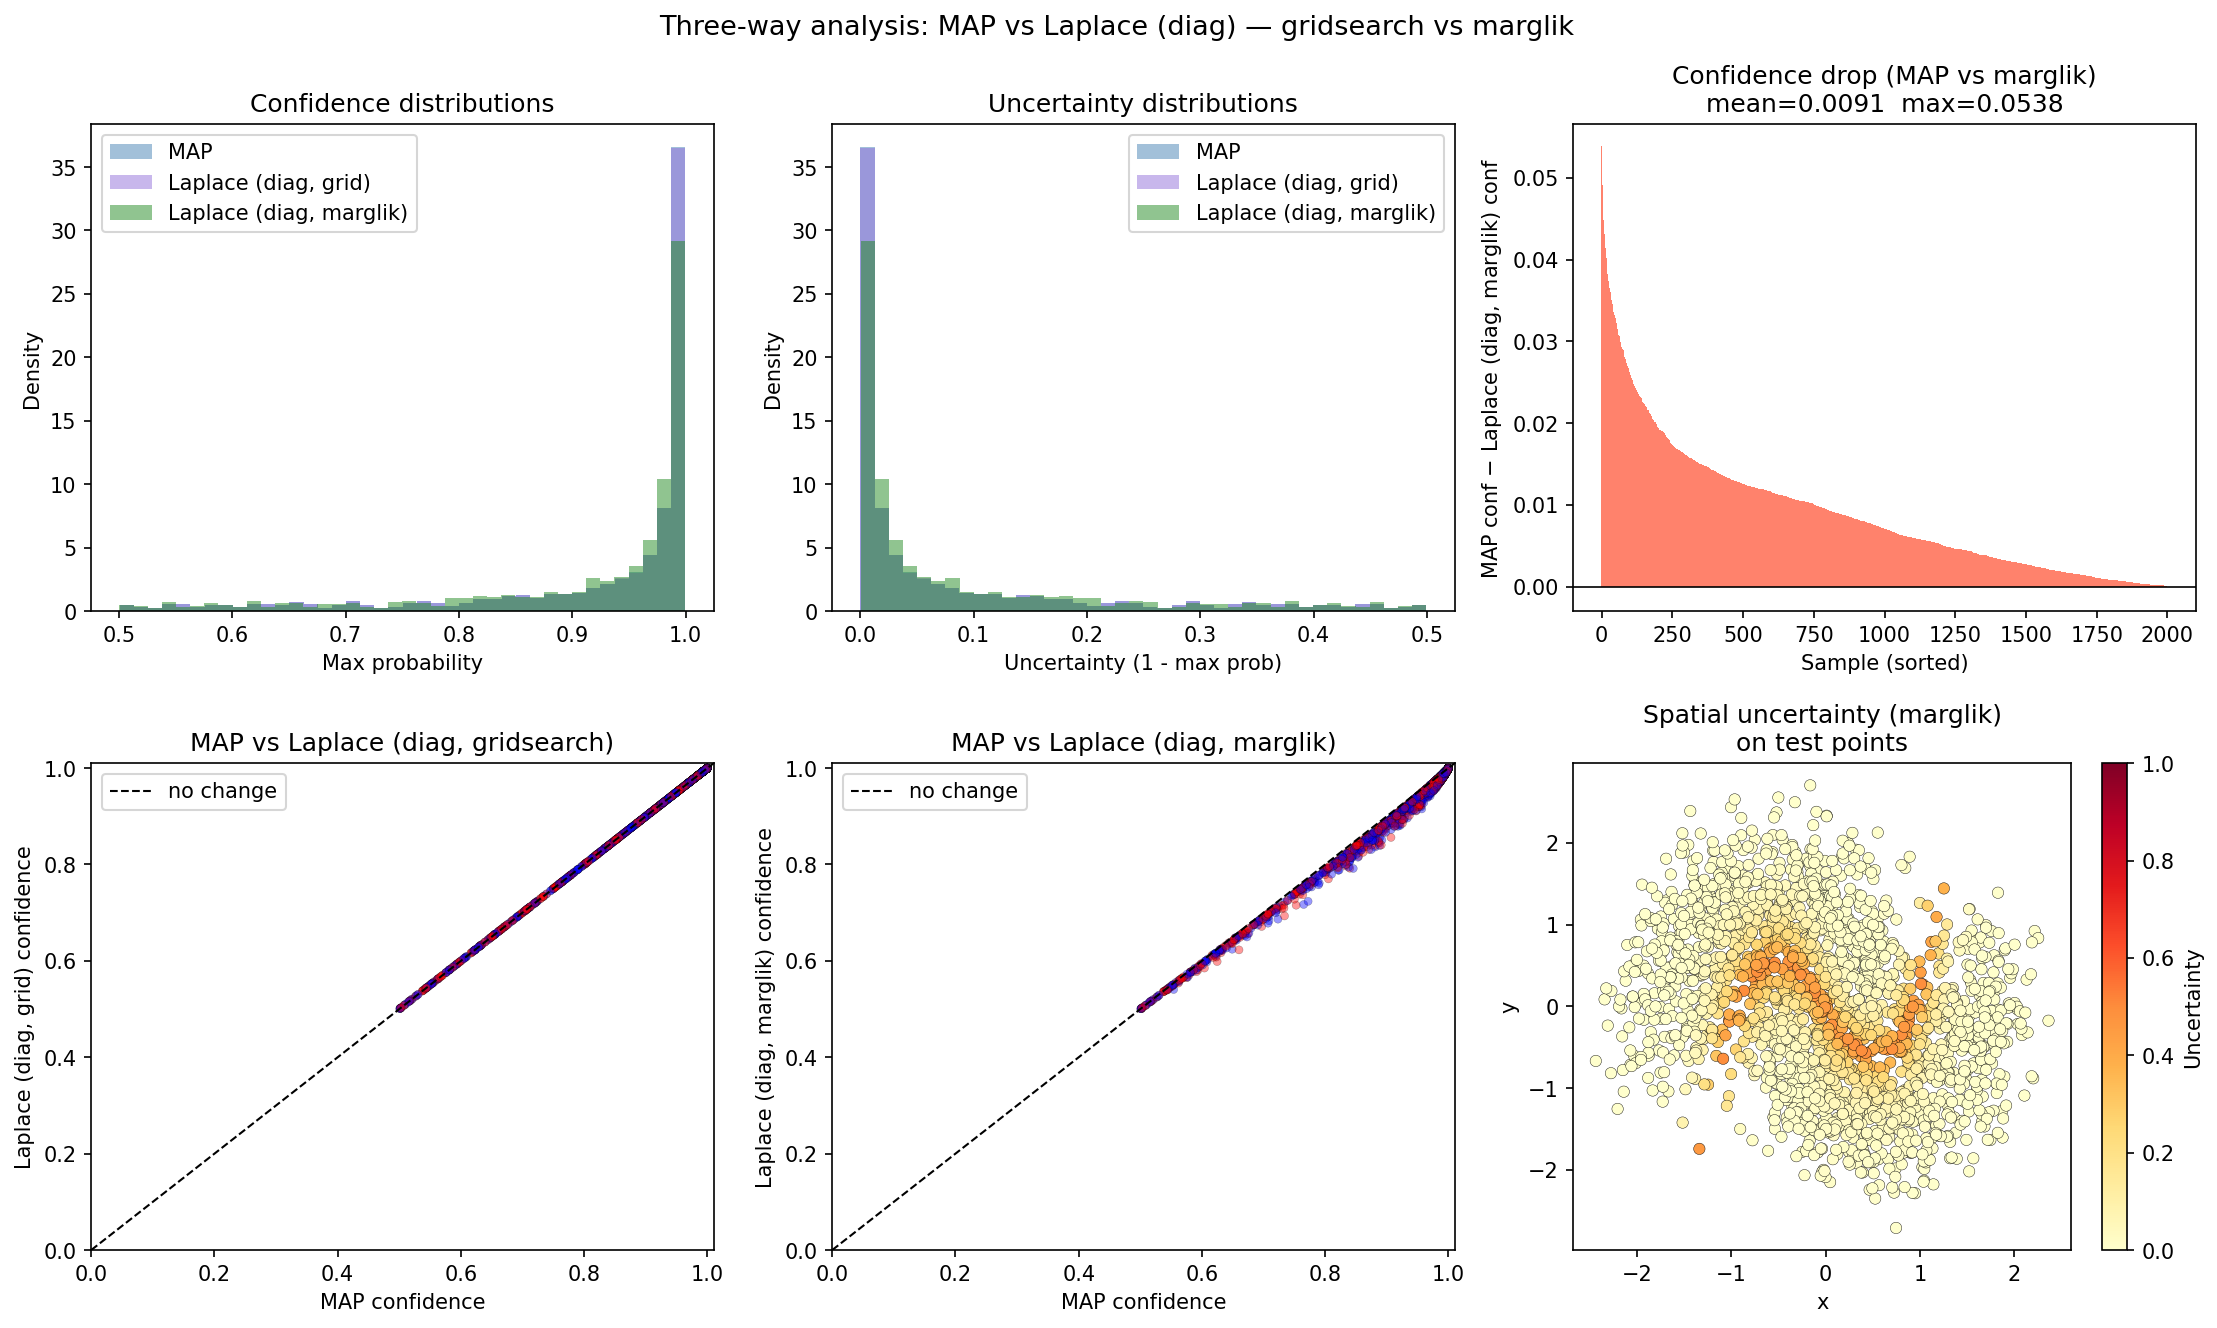
\includegraphics[width=0.45\textwidth]{./laplace_torch/figures/09_three_way_analysis.png}
\caption{Three-way analysis}
\end{figure}

\begin{figure}[h]
\centering
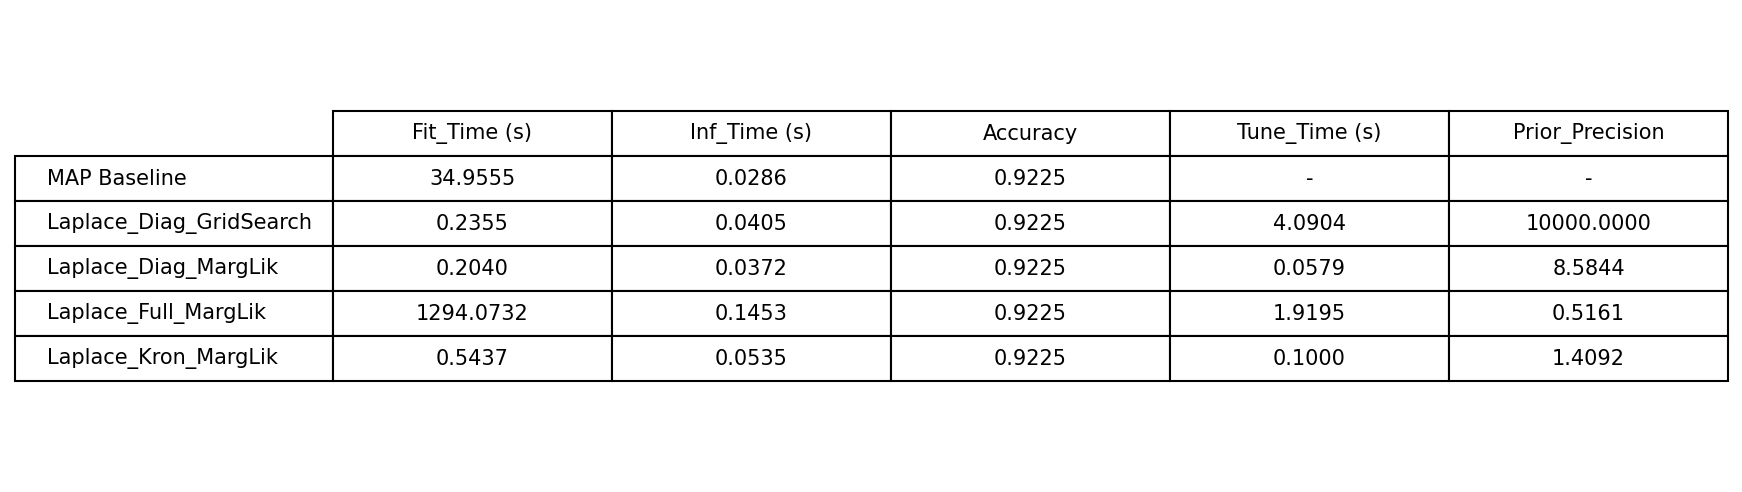
\includegraphics[width=0.45\textwidth]{./laplace_torch/figures/16_metrics_table.png}
\caption{Metrics comparison table}
\end{figure}

\clearpage

\section{Key Results}

\subsection{Sinusoid Results}
\begin{itemize}
\item Laplace RMSE: 1.4153
\item Laplace NLL: 1.5037
\item Laplace Cal Error: 0.0582
\item Bayesian-Torch RMSE: 1.0942
\item Bayesian-Torch NLL: 1.4853
\item Bayesian-Torch Cal Error: 0.0181
\end{itemize}

\subsection{PovertyMap Results (5-fold average)}
\begin{itemize}
\item Laplace ID RMSE: 0.4265
\item Laplace ID NLL: 0.5669
\item Laplace OOD RMSE: 0.5374
\item Laplace OOD NLL: 0.8642
\item Bayesian-Torch ID RMSE: 0.4193
\item Bayesian-Torch ID NLL: 37.1253
\item Bayesian-Torch OOD RMSE: 0.5544
\item Bayesian-Torch OOD NLL: 56.8239
\end{itemize}

\section{Library Usage Summary}

\subsection{Using Laplace-Torch}
\begin{itemize}
\item Train standard NN (MAP)
\item la = Laplace(model, "regression", subset\_of\_weights="all", hessian\_structure="full")
\item la.fit(train\_loader)
\item Optimize: la.log\_marginal\_likelihood(prior\_prec, sigma)
\item Predict: mu, var = la(X\_test)
\end{itemize}

\subsection{Using Bayesian-Torch}
\begin{itemize}
\item Train deterministic NN (MAP)
\item Set bnn\_prior\_parameters
\item dnn\_to\_bnn(model, params)
\item Train with ELBO: mse + kl / batch\_size
\item Predict: stack([model(X) for \_ in range(n\_mc)])
\end{itemize}

\end{document}